\documentclass[11pt]{standalone}

\usepackage{ifthen}
\usepackage{tikz} 
\usetikzlibrary{shapes.misc}
\usetikzlibrary{arrows,arrows.meta}
\usetikzlibrary{calc,intersections, patterns, math}

\definecolor{pfeil}{RGB}{168,167,167}
\definecolor{petrol}{RGB}{0, 118, 136}
\definecolor{darkgoldenrod}{RGB}{184, 134, 11}
\colorlet{petrol-lighter}{petrol!40}
\colorlet{darkgoldenrod-lighter}{darkgoldenrod!40}

\begin{document}

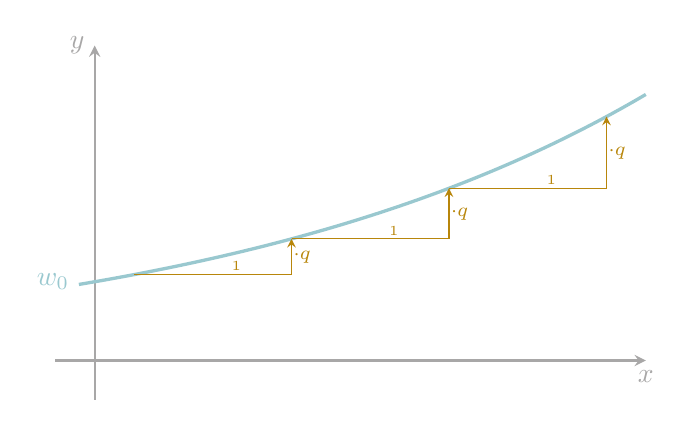
\begin{tikzpicture}[pfeil]

    % \draw[thick, fill=petrol!20, draw=petrol-lighter, rounded corners=2ex, opacity=0.5] (0,0) rectangle ++ (1.5,3.5);
    % \draw[thick, fill=darkgoldenrod!20, draw=darkgoldenrod-lighter, rounded corners=2ex, opacity=0.5] (5,0) rectangle ++ (1.5,3.5);

    \draw[thick, -stealth] (-0.5,0) -- (7,0) node[below]{$x$};
	\draw[thick, -stealth] (0,-0.5) -- (0,4) node[left]{$y$};
	
	\draw[very thick,domain=-0.2:7, smooth, samples=50, petrol-lighter] plot(\x,{1.19^\x});

	\foreach \x in {0.5,2.5,4.5}{
		\draw[darkgoldenrod, -stealth] (\x,{1.19^\x}) -- node [above, yshift=-0.75mm, xshift=3mm] {$\scriptscriptstyle 1$} ++(2,0) -- node[right, xshift=-1mm] {$\scriptstyle \cdot q$} (\x+2, {1.19^(\x+2)});
	}

	\node[left, petrol-lighter] at (-0.2,1) {$w_0$};

\end{tikzpicture}

\end{document}
